\documentclass[12 pt]{article}

\usepackage[affil-it]{authblk}
\usepackage{amsmath}
\usepackage{amssymb}
\usepackage{graphicx}
\usepackage[letterpaper, margin=2.20cm]{geometry}
\usepackage{float}
\usepackage{etoolbox}
\usepackage[font=small,labelfont=bf]{caption}

\makeatletter
\patchcmd{\@maketitle}{\LARGE \@title}{\fontsize{16}{19.2}\selectfont\@title}{}{}
\makeatother


\renewcommand\Authfont{\fontsize{12}{14.4}\selectfont}
\renewcommand\Affilfont{\fontsize{9}{10.8}\itshape}

\setcounter{topnumber}{2}
\setcounter{bottomnumber}{2}
\setcounter{totalnumber}{4}
\renewcommand{\topfraction}{0.85}
\renewcommand{\bottomfraction}{0.85}
\renewcommand{\textfraction}{0.15}
\renewcommand{\floatpagefraction}{0.8}
\renewcommand{\textfraction}{0.1}
\setlength{\floatsep}{5pt plus 2pt minus 2pt}
\setlength{\textfloatsep}{5pt plus 2pt minus 2pt}
\setlength{\intextsep}{5pt plus 2pt minus 2pt}


\begin{document}

%Title of paper
\title{\vspace{-1.5cm}\textbf{Fiber Integrated Nitrogen Vacancy Probes: Magnetic Gradiometry and Stimulated Fluorescence Quenching}}

\date{}

\author{\underline{Joe Becker}}
\author{Sean Blakley}
\author[1,2,3]{Ilya Fedotov}
\author[1,2,3]{Andrey Fedotov}
\author[1,2,3]{Aleksei M. Zheltikov}

\begin{small}
\affil{Department of Physics and Astronomy, Texas A\&M University, College Station, TX 77843-4242 USA}
\affil[2]{Physics Department, Intl. Laser Center, M. V. Lomonosov Moscow State University, Moscow 119992, Russia}
\affil[3]{Russian Quantum Center, Skolkovo, Moscow Region 143025, Russia}
\end{small}

\maketitle

\thispagestyle{empty}
\vspace{-1cm}
Nitrogen-vacancy (NV) color centers in diamond have proven to be a robust solid-state quantum system. We leverage 
this unique system, which allows us to manipulate and polarize an electron spin at room temperature using optical 
radiation, to create a compact dual core fiber magnetic gradiometry probe. Magnetic gradiometry measurements have
the advantage that they are insensitive to spatially uniform magnetic field backgrounds 
while still allowing high-spatial resolution measurements of variations in magnetic fields. 
Our previous work used two separate fibers to preform gradiometry measurements with a spatial resolution of 
0.5 mm \cite{Blakley2015}. By integrating the two fibers into a single dual core photonic crystal fiber 
(see Fig. \ref{fig:DualCore}) we have increased the spatial resolution of our gradiometry measurements to 4 microns.

We also are reporting an observed stimulated fluorescence quenching seen in our system when we illuminate the NV
diamond with infrared light \cite{Blakley2016}. We see that an increase in infrared power results in a decrease in
ODMR photoluminescence (see Fig. \ref{fig:FluorQuen}). This result can open a path toward a novel stimulated emission 
depletion (STED) regime for super-resolution microscopy.

\begin{figure}
    \centering
    \begin{minipage}{0.6\textwidth}
    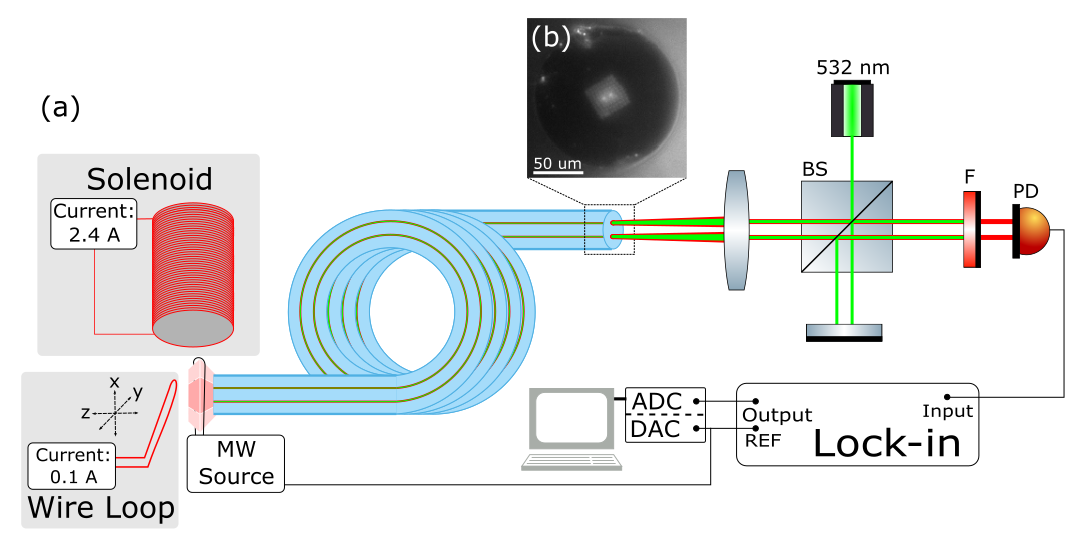
\includegraphics[width = 1.0\textwidth]{Images/DualCore.png}
    \caption{(a) A schematic of the dual core fiber gradiometry experiment. We used a beam splitter (BS) to split 
    the ND:YAG 532 nm pump laser into each fiber core. The NV fluorescence was collected using the same fiber then isolated using a long-pass filter (F) 
    and collected on a photodiode (PD). The optically detected magnetic resonance (ODMR) spectrum was measured using
lock-in detection observed as dips in NV fluorescence collected at PD. (b) An image of the dual core photonic crystal fiber with 4 $\mu$m spacing between cores.}
    \label{fig:DualCore}
    \end{minipage}
    \qquad
    \begin{minipage}{0.3\textwidth}
    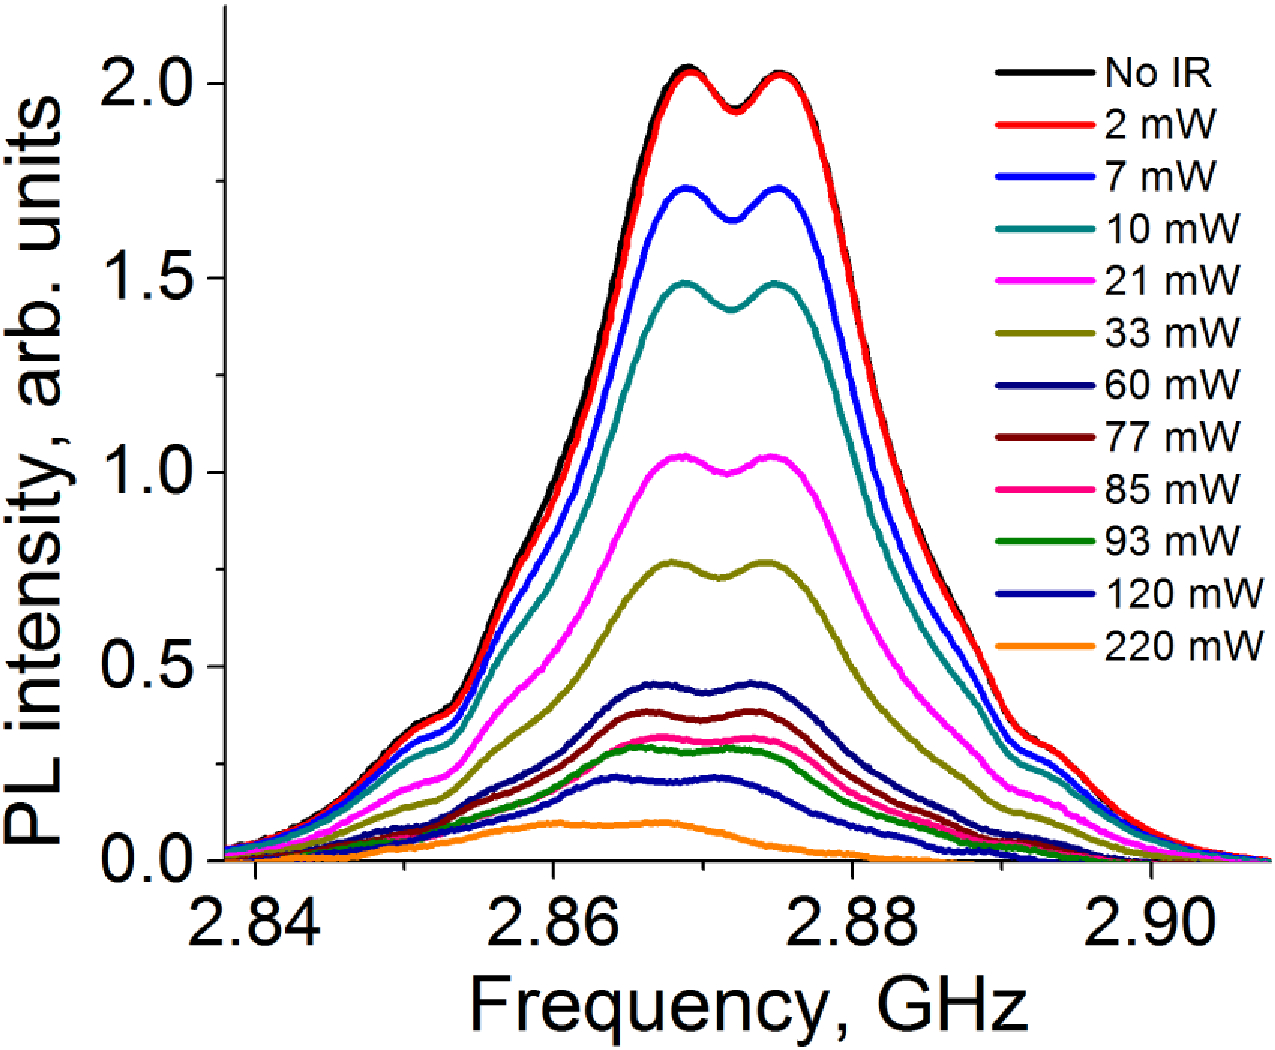
\includegraphics[width = 1.0\textwidth]{Images/FluorQuen.jpg}
    \caption{NV ODMR spectra measured in the presence of both the 532 nm pump and infrared radiation. We keep the 
    pump power constant and vary the infrared power from 2 to 220 mW. Fluorescence quenching is seen as infrared
    power increases.}
    \label{fig:FluorQuen}
    \end{minipage}
\end{figure}



\begingroup
\begin{scriptsize}

\renewcommand{\section}[2]{}%
\bibliographystyle{unsrt}
%\renewcommand{\chapter}[2]{}% for other classes
\bibliography{Abstract}
	%\vspace{-4cm}
\end{scriptsize}
	%\vspace{-4cm}
\endgroup

	
%\bibliography{pqe_poster2017}

\end{document}
